\subsection{Reporte de exploración de los datos}

\subsubsection*{Distribución del BCS y su relación con las métricas}

\begin{figure}[H]
  \centering
  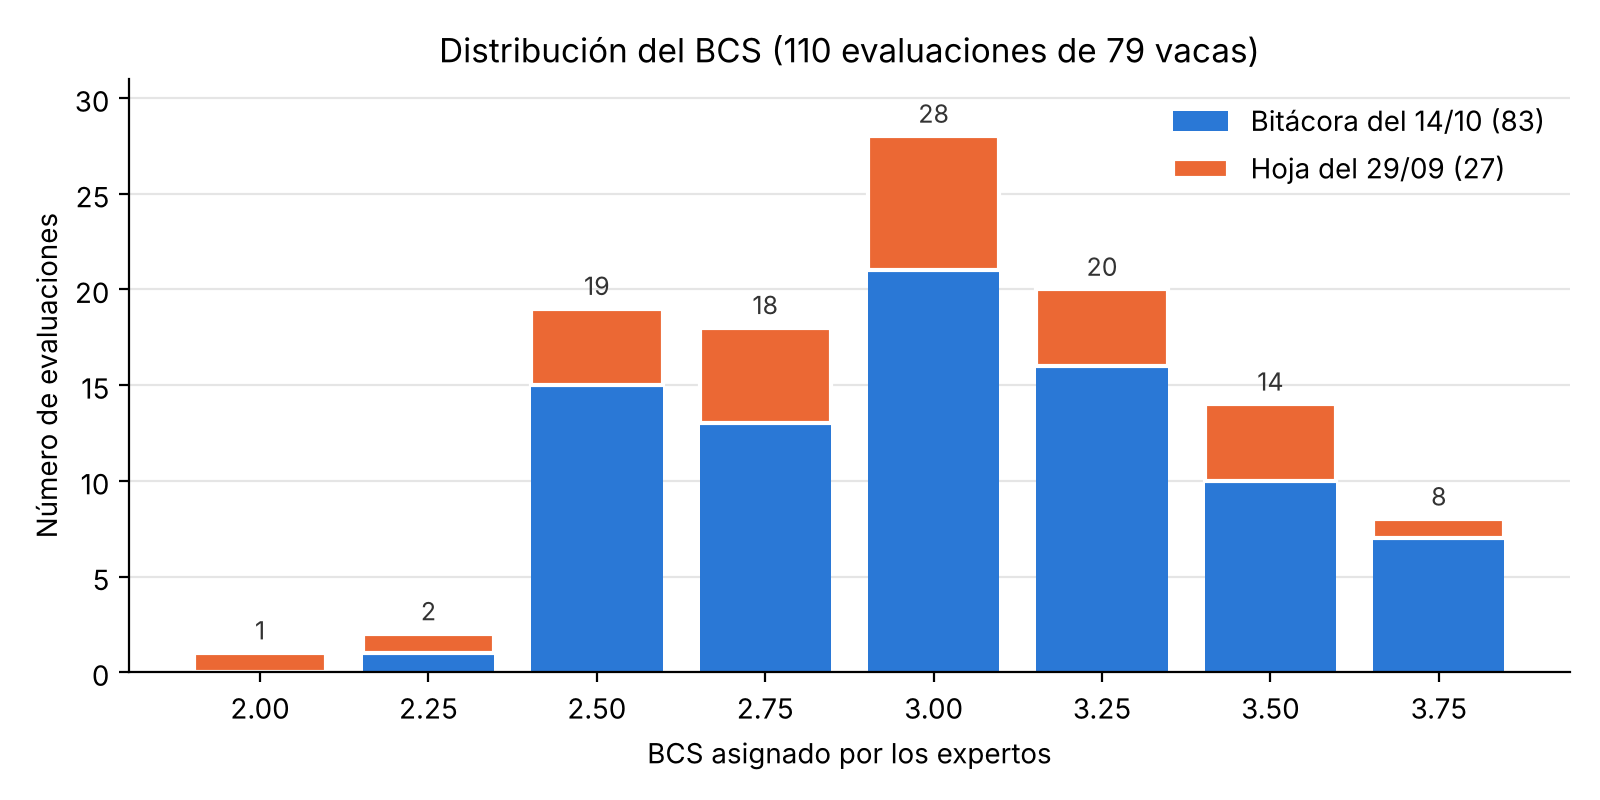
\includegraphics[width=0.85\textwidth]{figures/distribucion_bcs.png}
  \caption{Distribución del BCS asignado por los expertos.}
  \label{fig:distribucion-bcs}
\end{figure}

\begin{table}[H]
  \centering
  \caption{Evaluaciones por clase de BCS y fuente.}
  \label{tab:distribucion-bcs}
  \begin{tabular}{lrrrr}
    \toprule
    BCS & Bitácora 14/10 & Hoja 29/09 & Total & Porcentaje \\
    \midrule
    2.00 & 0 & 1 & 1 & 0.9\% \\
    2.25 & 1 & 1 & 2 & 1.8\% \\
    2.50 & 15 & 4 & 19 & 17.3\% \\
    2.75 & 13 & 5 & 18 & 16.4\% \\
    3.00 & 21 & 7 & 28 & 25.5\% \\
    3.25 & 16 & 4 & 20 & 18.2\% \\
    3.50 & 10 & 4 & 14 & 12.7\% \\
    3.75 & 7 & 1 & 8 & 7.3\% \\
    \midrule
    Total & 83 & 27 & 110 & 100\% \\
    \bottomrule
  \end{tabular}
\end{table}

La clase más frecuente es 3.0, con 28 evaluaciones (25.5\%). Las clases de los extremos tienen pocas evaluaciones, ya que 2.0 tiene 1, 2.25 tiene 2 y 3.75 tiene 8. No hay evaluaciones menores a 2.0 ni mayores a 3.75, así que el modelo no verá vacas fuera de ese rango.

Esta distribución es importante para las dos métricas que definimos. Con pocas vacas por clase, el porcentaje de predicciones dentro de $\pm0.25$ y $\pm0.50$ puede cambiar mucho con un solo error, y el MAE depende de qué tan lejos quedan las clases extremas del centro de la distribución.

\subsubsection*{Vacas con más de una evaluación}

En la bitácora del 14 de octubre hay 14 vacas con dos evaluaciones. La diferencia entre ellas es de 0.125 en promedio y de 0.25 como máximo, y en 7 vacas las dos evaluaciones son iguales. En la hoja hay 2 vacas con dos evaluaciones, la 1569 con una diferencia de 0.25 y la 1644 con evaluaciones iguales. Esto sirve como referencia de cuánto varía el BCS cuando lo asignan expertos distintos el mismo día.

Además, 15 vacas tienen BCS en las dos fechas. Entre el 29 de septiembre y el 14 de octubre su BCS difiere 0.225 en promedio (en valor absoluto) y 0.50 como máximo. En 5 vacas es igual y en 4 difiere más de 0.25, ya que la 1547 y la 1564 suben 0.5 del 29 de septiembre al 14 de octubre, la 1569 sube 0.375 y la 6137 baja 0.5. En conjunto no hay una tendencia, porque en promedio la hoja queda solo 0.008 por encima de la bitácora. Aun así, la diferencia máxima entre fechas (0.50) es el doble de la máxima entre expertos del mismo día (0.25), así que la fecha con la que se etiqueta cada foto importa.

\subsubsection*{Cruce entre fotos, conjunto de datos y BCS de expertos}

Cruzamos las 79 vacas con BCS con el conjunto de datos de VMS 3 (24 vacas) y con los datos de ordeño (34 vacas).

\begin{table}[H]
  \centering
  \caption{Cruce de las fuentes de datos.}
  \label{tab:cruce}
  \begin{tabular}{lr}
    \toprule
    Cruce & Vacas \\
    \midrule
    Con BCS de los expertos & 79 \\
    Con BCS y en VMS 3 & 20 \\
    Con BCS y con datos de ordeño & 12 \\
    En las tres fuentes & 2 (2082 y 8709) \\
    En VMS 3 sin BCS de los expertos & 4 (1570, 2165, 8769 y 91578) \\
    Con fotos y sin BCS & 2 (1549 y 1572) \\
    \bottomrule
  \end{tabular}
\end{table}

Las 20 vacas con BCS que están en VMS 3 son 1213, 1532, 1538, 1543, 1547, 1564, 1565, 1567, 1644, 2082, 2126, 2142, 6137, 6226, 8709, 8744, 8799, 91549, 91561 y 91576. Siete de ellas (1213, 1538, 1565, 1644, 2126, 6226 y 91576) solo tienen BCS de la hoja manuscrita.

De las 12 vacas con BCS de la bitácora que tienen valor en ``Evento BCS'', esta columna es mayor en 9, igual en 2 y menor en 1, y en promedio queda 0.43 puntos arriba. De las vacas que solo tienen BCS de la hoja, 4 tienen ``Evento BCS'', que es mayor en 3 e igual en 1. Como desconocemos qué mide esta columna, no se debe usar como si fuera el BCS de los expertos.

\subsubsection*{Relación con los datos de ordeño}

De las 34 vacas con datos de ordeño, 12 tienen BCS de los expertos, que son la 1204, 1221, 1554, 1624, 1634, 2076, 2082, 6178, 8709, 8729, 8758 y 8775. De ellas, solo la 2082 y la 8709 están también en VMS 3.

Los datos de ordeño siguen siendo contexto, porque cubren menos de la quinta parte de las vacas con BCS y sus fechas son de más de un año antes de las fotos. Por eso consideramos que su relación con el BCS no es significativa y no los usaremos como variables del modelo.

\subsubsection*{Exploración de los datos de ordeño (contexto)}

La tabla~\ref{tab:ordeno-resumen} resume las principales variables. La columna ``Global'' pondera a cada vaca por su número de ordeños. Las demás columnas comparan a las vacas entre sí y usan solo las 31 vacas con al menos 30 ordeños, porque tres vacas (1497, 8771 y 8775) tienen muy pocos datos para que sus promedios sean comparables.

\begin{table}[H]
  \centering
  \small
  \caption{Resumen de las variables de ordeño.}
  \label{tab:ordeno-resumen}
  \begin{tabularx}{\textwidth}{>{\raggedright\arraybackslash}Xrrrrr}
    \toprule
    Variable & Global & Media & Mediana & Mínimo & Máximo \\
    \midrule
    Ordeños por vaca & 7016 (34 vacas) & 206.4 & 244.5 & 1 & 419 \\
    Producción por ordeño (kg) & 13.72 & 13.53 & 13.86 & 7.66 & 18.85 \\
    Producción diaria (kg) & 31.12 & 30.45 & 28.13 & 13.15 & 55.50 \\
    Ordeños por día & 2.27 & 2.21 & 2.14 & 1.45 & 3.17 \\
    Duración media (min) & 8.48 & 8.24 & 7.83 & 5.36 & 13.51 \\
    Ordeños con patada (\%) & 18.5 & 18.2 & 15.2 & 0.7 & 62.2 \\
    Ordeños incompletos (\%) & 14.5 & 13.8 & 8.5 & 0.0 & 57.9 \\
    Ordeños con pezones no encontrados (\%) & 17.7 & 16.3 & 5.1 & 0.0 & 83.3 \\
    \bottomrule
  \end{tabularx}
\end{table}

La media, la mediana, el mínimo y el máximo son entre vacas. La producción diaria es la producción total entre los días en que la vaca tuvo al menos un ordeño.

\begin{figure}[H]
  \centering
  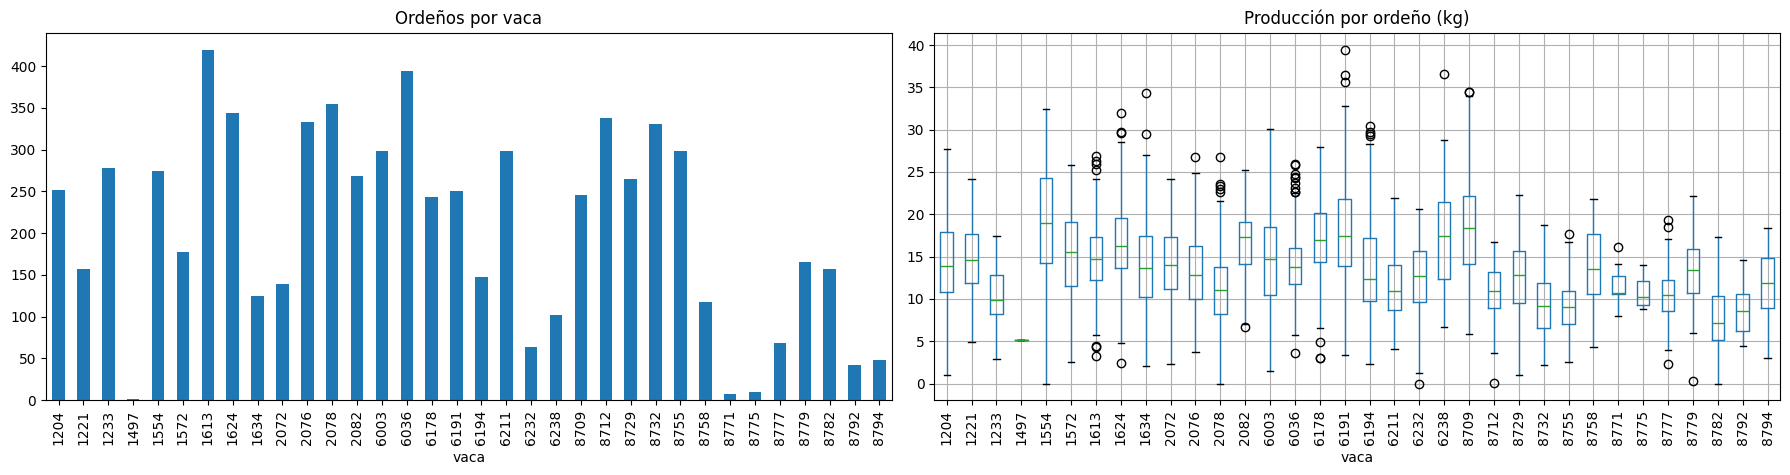
\includegraphics[width=\textwidth]{figures/ordenos_produccion_por_vaca.png}
  \caption{Ordeños por vaca y producción por ordeño (kg) de cada vaca.}
  \label{fig:ordenos}
\end{figure}

\begin{itemize}
  \item En producción, el promedio global fue de 13.7 kg por ordeño y la mediana entre vacas de 13.9 kg. La vaca con mayor promedio fue la 1554, con 18.9 kg por ordeño, y la de menor promedio entre las comparables fue la 8782, con 7.7 kg. Cinco vacas (1554, 2078, 6232, 8782 y 8712) tuvieron ordeños con 0 kg o 0.08 kg.
  \item En frecuencia y duración, las vacas se ordeñan en promedio 2.27 veces al día. El intervalo mediano entre ordeños va de 7.0 horas (vaca 6003) a 14.8 horas (vacas 8792 y 8794). Un ordeño dura en promedio 8.5 minutos. La vaca más rápida promedió 5.4 minutos (8712) y la más lenta 13.5 minutos (8755).
  \item Los incidentes se concentran en muy pocas vacas. Las vacas 8755, 8732 y 6003 tienen entre 45\% y 83\% de sus ordeños con pezones no encontrados o incompletos, y la 2076 tiene patada en el 62.2\% de sus ordeños.
  \item En la conductividad, la media por cuarto va de 3.82 mS/cm (TD) a 4.74 mS/cm (DD). Los ordeños con más de 6.0 mS/cm son pocos en todos los cuartos (entre 0.9\% y 2.8\%), pero se concentran en algunas vacas, como la 6178 en el cuarto DI (23.1\%).
  \item En cuanto a la sangre, solo 431 lecturas de cuarto tienen sangre mayor a 0 ppm, menos del 2\% del total.
  \item El estado AMD de la ubre vale 1 en 1050 de los 7016 ordeños (15.0\%). Por ahora solo consideramos su frecuencia, porque su significado debe confirmarse con el CAETEC.
  \item En cuanto a los robots, sobre las 7249 filas, VMS 3 registró 4276 (59.0\%), VMS 2 registró 1674 (23.1\%) y VMS 1 registró 1299 (17.9\%).
  \item En la cobertura temporal, 14 vacas tienen datos en prácticamente todo el rango de 140 días, 12 empiezan después del 01/03/2025 y 6 tienen ausencias prolongadas de entre 54 y 104 días. El socio formador explicó que esos huecos pueden corresponder al periodo seco de la vaca.
\end{itemize}

En cuanto al destino de la leche, la tabla~\ref{tab:destino} muestra a dónde fue la leche de los 7016 ordeños. Desviar la leche significa que su destino no es el tanque, donde se mezcla la leche de todas las vacas. Hubo 244 ordeños con leche desviada, de los cuales 152 fueron al drenaje y 92 a Divert 3. Según el socio formador, si la leche tiene sangre o microbios se desecha.

\begin{table}[H]
  \centering
  \caption{Destino de la leche.}
  \label{tab:destino}
  \begin{tabular}{lrr}
    \toprule
    Destino & Ordeños & Porcentaje \\
    \midrule
    Tanque & 6772 & 96.5\% \\
    Drenaje & 152 & 2.2\% \\
    Divert 3 & 92 & 1.3\% \\
    Total de ordeños & 7016 & 100\% \\
    \bottomrule
  \end{tabular}
\end{table}

Trece vacas enviaron menos del 95\% de su leche al tanque. El caso más destacable es la 6003, que solo envió el 71.5\% (213 de 298 ordeños). La columna ``Razón de la desviación'' tiene un único valor en todo el conjunto, así que no explica los 244 ordeños desviados.
